\documentclass[10pt]{article}

\usepackage{amsmath,amssymb}
\usepackage{graphicx}
\usepackage{caption}
\usepackage[margin=1.25in]{geometry}
\usepackage[english]{babel}
\usepackage[utf8]{inputenc}
\usepackage{array}
\usepackage{multirow}
\usepackage{algorithm}
\usepackage[noend]{algpseudocode}

\title{Computational Intelligence in Engineering\\Project A: Gait Analysis}
\author{Christopher Welter\\420078}
\date{September 14, 2021}

\begin{document}

\maketitle

\section{Introduction}

The aim of this project is to create a model of a person's gate through the use of neural networks. The collection of gait data will be accomplished using smartphone devices and using the Pyphox application. Several types of walking situations will be analyzed for 4 of the group members. Blabla, add onto this later when we know the further steps

\section{Data}
\subsection{Data Gathering}

The first important part of creating neural networks is the gathering of data. For each of the test subjects, 4 smarphones will be placed in 4 seperate locations as shown in the figure below:

\begin{center}
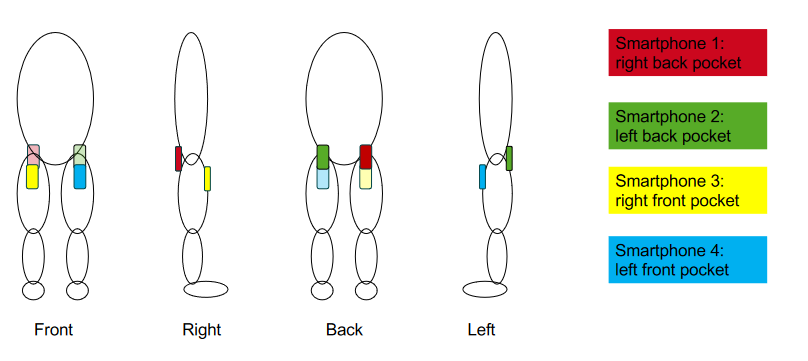
\includegraphics[scale=0.8]{C:/Users/chris/OneDrive/Documents/University/Aachen/Semester 3/CIE/Project A/Figures/smartphonelocations.PNG}
\captionof{figure}{Smartphone locations.[1]}
\end{center}

The location and amount of the smartphones allows for a more accurate capturing of a person's gait, as each leg acceleration is carefully captured. 3 experiments were conducted, and for 2 trials for each person. The following experiment procedures are found below:

\subsubsection{Experiment 1 Procedure}
\begin{enumerate}
\item Place phones into the relevant positions as shown in Figure 1.
\item Begin the Pyphox application and begin the recording data procedure.
\item Stand still for a few seconds.
\item Walk 30 seconds in a straight line at a normal speed.
\item After walking for 30 seconds, stop the data recording and application.
\item Store the final data in csv format.
\end{enumerate}

\subsubsection{Experiment 2 Procedure}
\begin{enumerate}
\item Place phones into the relevant positions as shown in Figure 1.
\item Begin the Pyphox application and begin the recording data procedure.
\item Stand still for a few seconds.
\item Walk up 10(at least) steps at a normal speed.
\item After walking up the steps, stop the data recording and application.
\item Store the final data in csv format.
\end{enumerate}

\subsubsection{Experiment 3 Procedure}
\begin{enumerate}
\item Place phones into the relevant positions as shown in Figure 1.
\item Begin the Pyphox application and begin the recording data procedure.
\item Stand still for a few seconds.
\item Add an impariment device(small cube or rock) in the right shoe.
\item Walk 30 seconds in a straight line at a normal speed.
\item After walking for 30 seconds, stop the data recording and application.
\item Store the final data in csv format.
\end{enumerate}

\subsection{Data Preprocessing}

After gathering the relevant data for each subject, the data must be processed in several ways. Rather than repeating te above experiments twice, we simply left the recording running and repeated the previous steps. The data was then split in half and we are left with the following form:

\begin{center}
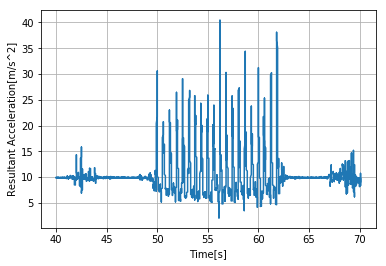
\includegraphics[scale=0.8]{C:/Users/chris/OneDrive/Documents/University/Aachen/Semester 3/CIE/Project A/Figures/exampleRawAcceleration.png}
\captionof{figure}{Example Acceleration Output}
\end{center}



\section{Bibliography}
[1] - presentations
\end{document}


